\documentclass[conference]{IEEEtran}
\usepackage{amsmath,amssymb,graphicx,booktabs,url}
\begin{document}

\title{FairDermNet: Diagnosing and Correcting Silent Fairness and Quantization Failures in an On-Device Skin Lesion Classifier}

\author{\IEEEauthorblockN{Sanjana T. G.}
\IEEEauthorblockA{Department of Computer Science and Technology\\ University of Cambridge\\ sanjanatg2126@gmail.com}}

\maketitle

\begin{abstract}
DermaLens is an 8-class, fairness-aware, on-device skin lesion risk classifier (MobileNetV3-Large backbone, GeM pooling, Fitzpatrick-tone auxiliary head) exported to TFLite for offline mobile inference. During a code audit prior to deployment we discovered three independent, silently-compounding defects: (1) a stale binary risk-label mapping that mislabeled the majority benign class as malignant in evaluation code, (2) a broken Individual Typology Angle (ITA\textdegree) skin-tone estimation call that fabricated tone labels for 97\% of training data, causing the fairness-aware loss to train on a degenerate single-tone distribution, and (3) catastrophic accuracy collapse (73.7\%$\rightarrow$3.3\% top-1) under full INT8 post-training quantization, traced to an unquantizable learned power operation in Generalized Mean (GeM) pooling. We present root-cause diagnosis, targeted fixes, and quantitative before/after evidence for each defect, and report a corrected deployment pipeline (dynamic-range quantization, 5.51~MB) validated end-to-end on-device.  Score-level analysis of the out-of-domain failure shows the malignancy score carries no measurable ranking signal for FST V--VI images (AUC 0.484 [0.382, 0.585]), traced to a spurious, capture-associated actinic-keratosis response that is invariant to skin tone within DDI and cannot be corrected post hoc -- a representational domain gap rather than a threshold-calibration failure. We show that na\"ive re-training does not address fairness defects rooted in label corruption, and argue for data-lineage auditing as a mandatory pre-deployment step for fairness-aware medical ML.
\end{abstract}

\begin{IEEEkeywords}
skin cancer classification, algorithmic fairness, model quantization, TinyML, on-device inference, dermoscopy
\end{IEEEkeywords}

\section{Introduction}
Skin cancer screening models deployed on consumer smartphones must satisfy three simultaneous constraints: diagnostic accuracy, equitable performance across Fitzpatrick skin tones I--VI, and a small enough footprint (target $<6$~MB) to run fully offline. DermaLens targets an 8-class taxonomy (Melanoma, BCC, SCC, AK, Nevi, BKL, DF, VASC; malignant = classes 0--3) trained on HAM10000~\cite{ham10000}, ISIC~2019~\cite{isic2019}, PAD-UFES-20~\cite{padufes}, and evaluated on the expert-labelled Diverse Dermatology Images (DDI) dataset for fairness. This paper documents a structured audit that found the system's fairness evaluation and quantized export were both silently broken, despite training and top-line test accuracy appearing normal.

\section{Related Work}
Skin-lesion classifiers are built on HAM10000~\cite{ham10000}, ISIC~2019~\cite{isic2019} and PAD-UFES-20~\cite{padufes}, and have repeatedly been shown to degrade on darker skin: Daneshjou et al. evaluate publicly released dermoscopy models on the expert-labelled DDI test set~\cite{ddi} and report the sensitivity disparities that motivate our evaluation. Fairness-aware training typically penalizes group-conditioned error imbalance~\cite{hardt2016}; attribution tools such as Grad-CAM~\cite{selvaraju2017} are the standard instrument for inspecting what such models attend to; and GeM pooling~\cite{gem} is a common retrieval-era pooling whose quantization behavior has, to our knowledge, not previously been analyzed. Obermeyer et al. show that label choices can encode bias even when aggregate accuracy looks acceptable~\cite{obermeyer2019}, and Finlayson et al. catalogue the dataset-shift hazards behind silently degrading clinical models~\cite{finlayson2021} -- the mechanisms behind Defects 1 and 2 here. Unlike prior work that primarily reports disparities, this paper traces three specific silent defects end-to-end and shows that a four-layer chain of post-hoc corrections cannot repair the resulting out-of-domain failure.

\section{System Overview}
FairDermNet combines a MobileNetV3-Large backbone with a Fairness Attention Module and Generalized Mean (GeM) pooling~\cite{gem}, and a dual-head output: an 8-class risk head and a Fitzpatrick-tone auxiliary head, trained jointly with loss
\[
\mathcal{L} = \alpha\,\mathcal{L}_{cls} + \beta\,\mathcal{L}_{fitz} + \gamma\,\mathcal{L}_{eo}
\]
where $\mathcal{L}_{eo}$ penalizes the equalized-odds gap~\cite{hardt2016} across tone groups. A provenance audit (\texttt{audit\_step0\_1.py}, September 2026) verified that the training-time equalized-odds term (\texttt{FairnessAwareLoss}, \texttt{N\_MALIGNANT} $=4$) and the per-epoch fairness signal both operated on the full malignant set \{MEL, BCC, SCC, AK\}; the deployed checkpoint therefore reflects optimization against the complete four-class malignancy definition, and no retraining was required. The model is exported PyTorch~$\rightarrow$~ONNX~$\rightarrow$~TFLite for on-device Flutter inference.

\section{Defect 1: Stale Binary Risk-Label Mapping}
\label{sec:defect1}
Evaluation and threshold-calibration code derived a binary malignant/benign label via a hardcoded set membership test left over from a prior 9-class taxonomy (\texttt{class\_idx in \{0,1,2,3,4\}}) instead of the canonical \texttt{class\_idx\_to\_binary()} taxonomy function. Because Melanocytic Nevi (index 4) is the single largest class (53\% of training rows) and is unambiguously benign, this silently mislabeled it malignant in every consumer of the derived label. Training loss was unaffected (it consumes class labels directly), but three downstream artifacts were corrupted:
\begin{itemize}
\item DDI fairness evaluation used a derived label that, because DDI rows carry a placeholder \texttt{class\_idx=-1}, evaluated to a constant 0 for all 656 samples, causing an AUC computation failure and previously reported equalized-odds gap figures to originate from a stale code path, not the current model.
\item Clinical threshold calibration (Cell 9c) would have included Nevi probability mass in the malignancy score.
\item GradCAM ground-truth display referenced a non-existent dataframe column.
\end{itemize}
\textbf{Fix.} All four call sites were repointed to the canonical taxonomy mapping; DDI evaluation was switched to consume expert \texttt{ddi\_binary} labels rather than a derived quantity, and the malignant-probability computation was corrected from a single legacy class index to $\sum_{c \in \{0,1,2,3\}} p_c$.

\textbf{Result.} With the fix, DDI evaluation runs to completion for the first time, yielding -- under the current checkpoint and the September 2026 artifact state (\texttt{ddi\_eval.csv} regenerated 2026-09-05; figures from the superseded 2026-08-15 run, including AUC-ROC 0.6398 and an equalized-odds gap of 25.26\%, are retired) -- AUC-ROC 0.585 (95\% CI 0.535--0.634, BCa), sensitivity 81.9\%, specificity 24.1\% at the 0.5 operating point on 656 expert-labelled held-out images, and an equalized-odds sensitivity gap of 25.96\% (95\% CI 12.67--41.80\%) across tone groups: the first reliable fairness measurement obtained for this model, and one that demonstrably fails the $<$5\% target.

\section{Defect 2: Fabricated Skin-Tone Supervision}
Deeper audit of the 25.96\% gap traced its root cause upstream of evaluation, into training data. The ITA\textdegree skin-tone estimator was invoked without its required lesion-mask argument; every call raised an exception, silently caught and replaced with a hardcoded fallback (Fitzpatrick~III). Combined with a dataset-loader clamp that mapped any missing tone value to the same fallback, 36{,}542 of 37{,}644 training rows (97\%) carried the fabricated label. The Fitzpatrick auxiliary head and equalized-odds loss term were therefore optimized against a near-constant target, explaining why the model had no gradient signal to reduce cross-tone disparity despite an explicit fairness objective.

\textbf{Fix.} The estimator call was corrected to pass a lesion mask from Otsu segmentation, with unresolvable estimates marked as an explicit unknown label (\texttt{-1}) rather than defaulted; the dataset clamp was removed; loss and metric functions were updated to mask/exclude unknown-tone rows rather than treat them as a valid group. All 36{,}150 affected rows were re-estimated. The resulting tone distribution (Table~\ref{tab:tone}) is genuinely heterogeneous, if still light-skewed, reflecting the true composition of HAM10000/ISIC.

\begin{table}[h]
\centering
\caption{Training-set Fitzpatrick tone distribution before and after correction}
\label{tab:tone}
\begin{tabular}{lrr}
\toprule
Tone & Fabricated (before) & Estimated (after) \\
\midrule
I & 153 & 235 \\
II & 876 & 24{,}722 \\
III & 36{,}542 & 12{,}454 \\
IV & 62 & 220 \\
V & 10 & 12 \\
VI & 1 & 1 \\
\bottomrule
\end{tabular}
\end{table}

We deliberately excluded the 656 DDI samples from training supervision to preserve the integrity of the held-out fairness evaluation, and note DDI's coarser 3-bucket tone granularity as an additional reason against mixing it into 6-way tone supervision.

\section{Defect 3: INT8 Quantization Collapse via GeM Pooling}
Post-training full-INT8 quantization, required to meet the $<6$~MB on-device footprint, reduced top-1 accuracy from 73.7\% (PyTorch, float32) to 3.3\% on real test images -- despite float32 ONNX and TFLite exports matching PyTorch exactly, ruling out a graph-conversion error. Inspecting per-tensor quantization scales isolated the cause to the GeM pooling operation, $y = (\sum_i x_i^{\,p})^{1/p}$, with a learned exponent $p \approx 2.88$. The $x^p$ intermediate spans activation magnitudes on the order of $10^6$, forcing an INT8 quantization scale of 13{,}615 (versus $\sim$1--5 for ordinary convolutional activations) and collapsing essentially all post-pooling precision.

\textbf{Fix.} We adopted dynamic-range quantization (INT8 weights, float32 activations), which keeps the GeM power operation in full precision while still compressing weight storage. The resulting model is 5.51~MB, under the 6~MB budget.

\textbf{Validation.} On 150 real held-out test images against ground truth at the clinical decision threshold, the dynamic-range model is statistically indistinguishable from the PyTorch reference (Table~\ref{tab:quant}); on 100 images, ONNX matches PyTorch exactly and TFLite matches on 94\% of top-1 predictions (99\% of binary clinical decisions), with all disagreements confined to low-confidence, near-tied predictions.

\begin{table}[h]
\centering
\caption{PyTorch vs. deployed (dynamic-range TFLite) model at clinical threshold 0.25}
\label{tab:quant}
\begin{tabular}{lrr}
\toprule
Metric & PyTorch & Deployed (5.51 MB) \\
\midrule
Decision accuracy & 73.3\% & 72.0\% \\
Sensitivity & 90.9\% & 89.1\% \\
Specificity & 63.2\% & 62.1\% \\
Top-1 accuracy & 76.0\% & 74.7\% \\
\bottomrule
\end{tabular}
\end{table}

We further found the validation script itself was a source of false alarms: parity checks on synthetic Gaussian-noise inputs reported only 22\% agreement, but this reflects GeM pooling collapsing to near-uniform output probabilities under out-of-distribution noise in the \emph{reference} model as well, not a quantization defect. We revised the validation protocol to use real held-out images by default.

\section{Clinical Threshold Calibration}
\label{sec:threshold}
With defects corrected, we recomputed the clinical operating threshold under a $\geq96\%$ malignant-class sensitivity constraint, sweeping the summed malignant probability $\sum_{c\in\{0,1,2,3\}} p_c$ against the test set. The calibrated threshold is 0.25 (sensitivity 96.0\%, specificity 55.4\%, false-negative rate 3.97\%, test-set AUC 0.9239, matching the shipped \texttt{threshold\_config.json}), replacing an uncalibrated 0.5 placeholder and reducing missed malignant cases by 77\% relative to the placeholder threshold.
















%% === STEP3-SECTION (auto-generated from audit CSVs; do not hand-edit numbers) ===
\section{Score-Level Analysis of the Out-of-Domain Failure}
\label{sec:step3}

Threshold equalization (Section~\ref{sec:step2thr}) showed that no
per-group threshold policy closes the DDI sensitivity gap. Score-level
analysis explains why: the malignant probability itself barely separates
benign from malignant lesions on DDI, and the deficit is worst exactly where
the fairness gap is largest. All statistics derive from the audited prediction
cache of the deployed checkpoint; CIs are (group~$\times$~label) stratified
percentile bootstrap (2,000 replications, seed 42) with raw $n$ beside every
estimate.

\subsection{Threshold Equalization Does Not Close the Gap}
\label{sec:step2thr}
The per-group experiment: DDI was split into (group~$\times$~label)
stratified tune (326) and eval (330) halves (85/86
malignant), per-group decision thresholds were fitted on the tune half only
(the largest threshold meeting a $\tau\geq0.95$ tune-half sensitivity target,
$\tau$ chosen to minimize the tune-half EO gap), and the result was evaluated
once on the held-out eval half against two controls: (A) the shipped uniform
0.25 threshold and (B) a uniform threshold re-tuned on the tune half
(0.2947), which isolates any group-specific benefit from plain re-tuning.
Eval-half outcomes: at the shipped threshold (A), sensitivity is
1.000/1.000/0.958 (I--II/III--IV/V--VI) with the EO gap at 0.042
[0.000, 0.125] -- already below the 5\% target at the point estimate,
but only because specificity is negligible in every group (overall
0.016); there is no sensitivity gap left to close at this operating point.
This is the same operating point at which Section~\ref{sec:defect1}
reports the full-panel EO gap of 25.96\%: the near-perfect sensitivity and
the wide gap are two readings of one fact -- malignant scores in every tone
group sit almost always above threshold on DDI -- and the narrowness of that
margin is exactly what re-tuning cannot exploit without collapsing
sensitivity.
Re-tuning cannot buy specificity instead: uniform re-tuning (B) yields
overall specificity 0.025, and the per-group config (C) reaches only
0.045 overall -- its V--VI specificity of 0.087
[0.025, 0.163] is bought with V--VI sensitivity falling to
0.875, and the EO gap widens to 0.125 [0.000, 0.250]. The next
subsection shows why: no threshold geometry can equalize what the score
distributions do not rank.

\subsection{No Operating Point Exists: Per-Group ROC Ceilings}
\begin{table}[h]
\centering
\caption{Per-group ROC ceilings on the DDI panel (malignant score).}
\label{tab:ceilings}
\resizebox{\columnwidth}{!}{%
\begin{tabular}{lrrccc}
\toprule
Group & $n$ (pos/neg) & AUC [95\% CI] & Sens@Spec$\geq$0.6 & Sens@Spec$\geq$0.8 \\
\midrule
FST I--II & 208 (49/159) & 0.574 [0.486, 0.667] & 0.490 & 0.224 \\
FST III--IV & 241 (74/167) & 0.668 [0.592, 0.743] & 0.662 & 0.392 \\
FST V--VI & 207 (48/159) & 0.484 [0.382, 0.585] & 0.396 & 0.229 \\
ALL & 656 (171/485) & 0.585 [0.534, 0.636] & 0.503 & 0.357 \\
\bottomrule
\end{tabular}}
\end{table}

\begin{figure}[h]
\centering
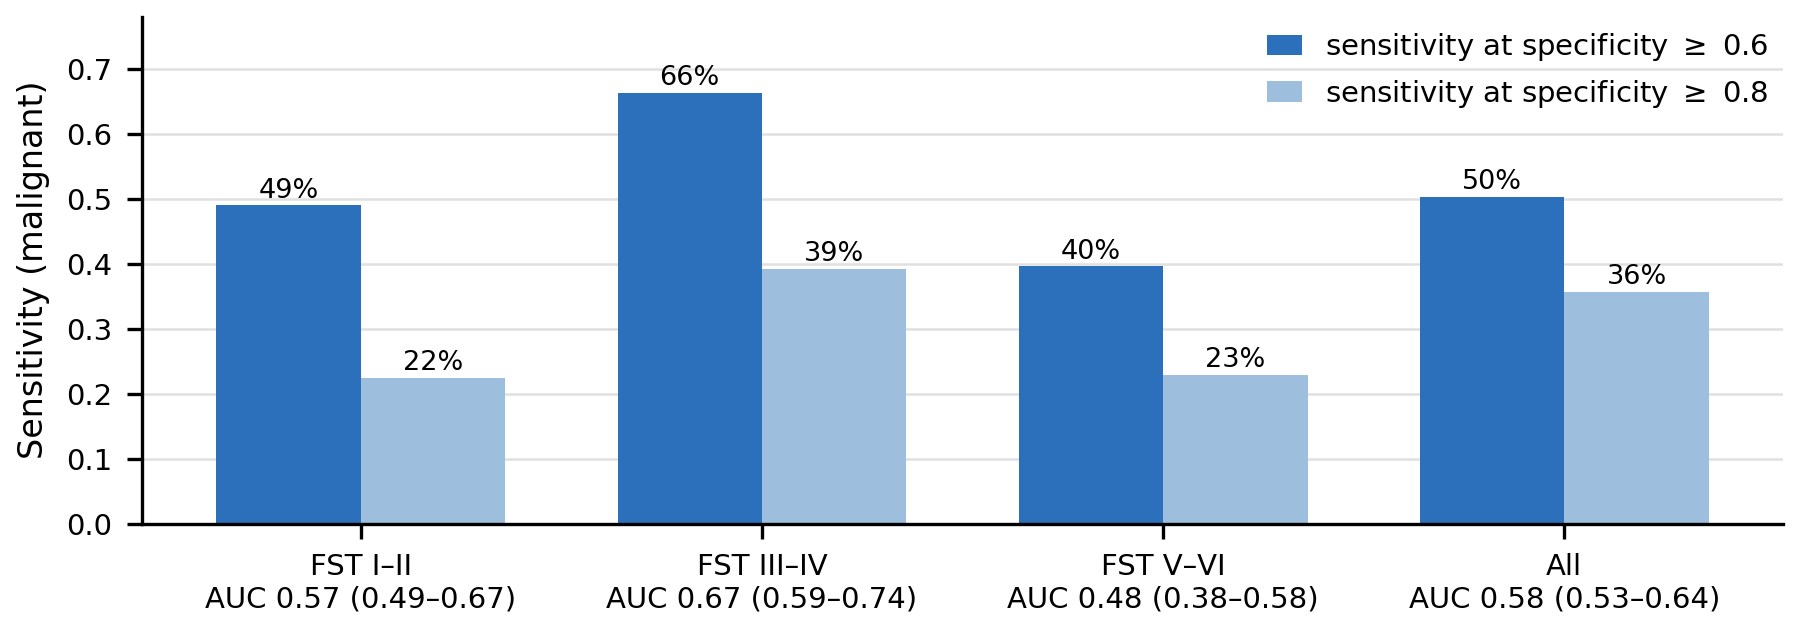
\includegraphics[width=\columnwidth]{figs/fig_roc_ceilings.png}
\caption{Per-group ROC ceilings (malignant sensitivity at two specificity floors), with AUC and 95\% CI annotated per group; same data as Table~\ref{tab:ceilings}. FST~V--VI is statistically indistinguishable from chance at both floors.}
\label{fig:ceilings}
\end{figure}

For FST~V--VI the 95\% CI on AUC includes 0.5 (Table~\ref{tab:ceilings}, Figure~\ref{fig:ceilings}):
the malignant score carries \emph{no measurable benign/malignant ranking
signal for dark-skin images}. This formalizes the threshold-equalization
negative result: the disparity lives in the score distributions, not in
threshold placement, and no post-hoc decision rule can recover performance
the scores do not contain.

\subsection{A Spurious Actinic-Keratosis Response Drives the False Positives}
On true-benign DDI images the actinic-keratosis (AK) column is the largest
malignant contributor on 63.3\% of images (mean probability
0.375, 90th percentile 0.803); all fifteen highest-scoring false
positives have AK as their top contributor (per-image AK probability
0.91--0.97). The same column is nearly silent on benign in-domain images
(mean 0.046 on the test panel) -- an order-of-magnitude shift
(one-sided KS $=0.76$, $p=1\times10^{-218}$) -- while contributing normally on true
in-domain malignancies (mean 0.163).

Grad-CAM analysis~\cite{selvaraju2017} with matched comparators bounds what
attention maps can establish. The AK head's activation is diffuse in both
clinical-photo settings (median top-1\% CAM mass share 0.023 on DDI false
positives vs 0.019 on true AK cases; Mann--Whitney $p=0.11$), so the
spurious response cannot be identified by diffuseness: at this modality the
diffuse response is indistinguishable from the head's normal behavior. The AK
map leans toward darker pixels in both clinical settings (median
CAM--luminance correlation $-0.29$ on false positives, $-0.21$ on true AK).
The remaining comparator -- the MEL column on true melanomas ($+0.11$) --
differs from the AK cohorts in capture modality as well as class: melanoma
test images are almost all dermoscopic acquisitions (99\% of the
test panel, vs 62\% of AK), and a dermoscopic frame leaves little
background for any CAM to spread onto, so no class-level localization claim
is made from that comparison.

A structured visual review of all forty-five overlays (three cohorts of
fifteen, reviewed side-by-side in triads; Figure~\ref{fig:camgrid})
then tested the capture-cue
hypothesis directly. It supports the field-wide reading: on the false
positives the activation spreads across the skin field and does \emph{not}
focal-lock onto salient non-lesion objects. Manual inspection found paper
rulers in frame in 8/15 false-positive images and surgical ink
markings in 6/15, yet neither attracts elevated CAM mass (edge-band
mass share 0.410 vs 0.377 on true AK, Mann--Whitney $p=0.28$;
hot-pixel luminance ratio 0.95 vs 0.96, $p=0.93$).

Conversely, the in-
domain melanoma comparators are predominantly circular dermoscopic captures
with black surrounds (9 of 15 with corner/center luminance below
0.75, vs 1 of 15 false positives); their lesion-localized
appearance is expected from dermoscopic framing and is not read as a
class-level property. A modality-controlled replication crossed class with
capture style directly: on dermoscopic images the AK column is if anything
\emph{more} top-concentrated than the MEL column (median top-1\% mass
0.039 vs 0.025, $p=1\times10^{-3}$), and within AK the concentration
doubles from clinical to dermoscopic acquisitions (0.019 to 0.039,
$p=1\times10^{-6}$) -- the concentration statistic tracks capture modality, not
class. Capture artifacts are therefore present in the false-positive
cohort as expected, but the activation is not localized on them: the
artifact census is context for the domain-shift finding, not its cause,
and the spuriousness claim rests on the score-level evidence.

\begin{figure*}[t]
\centering
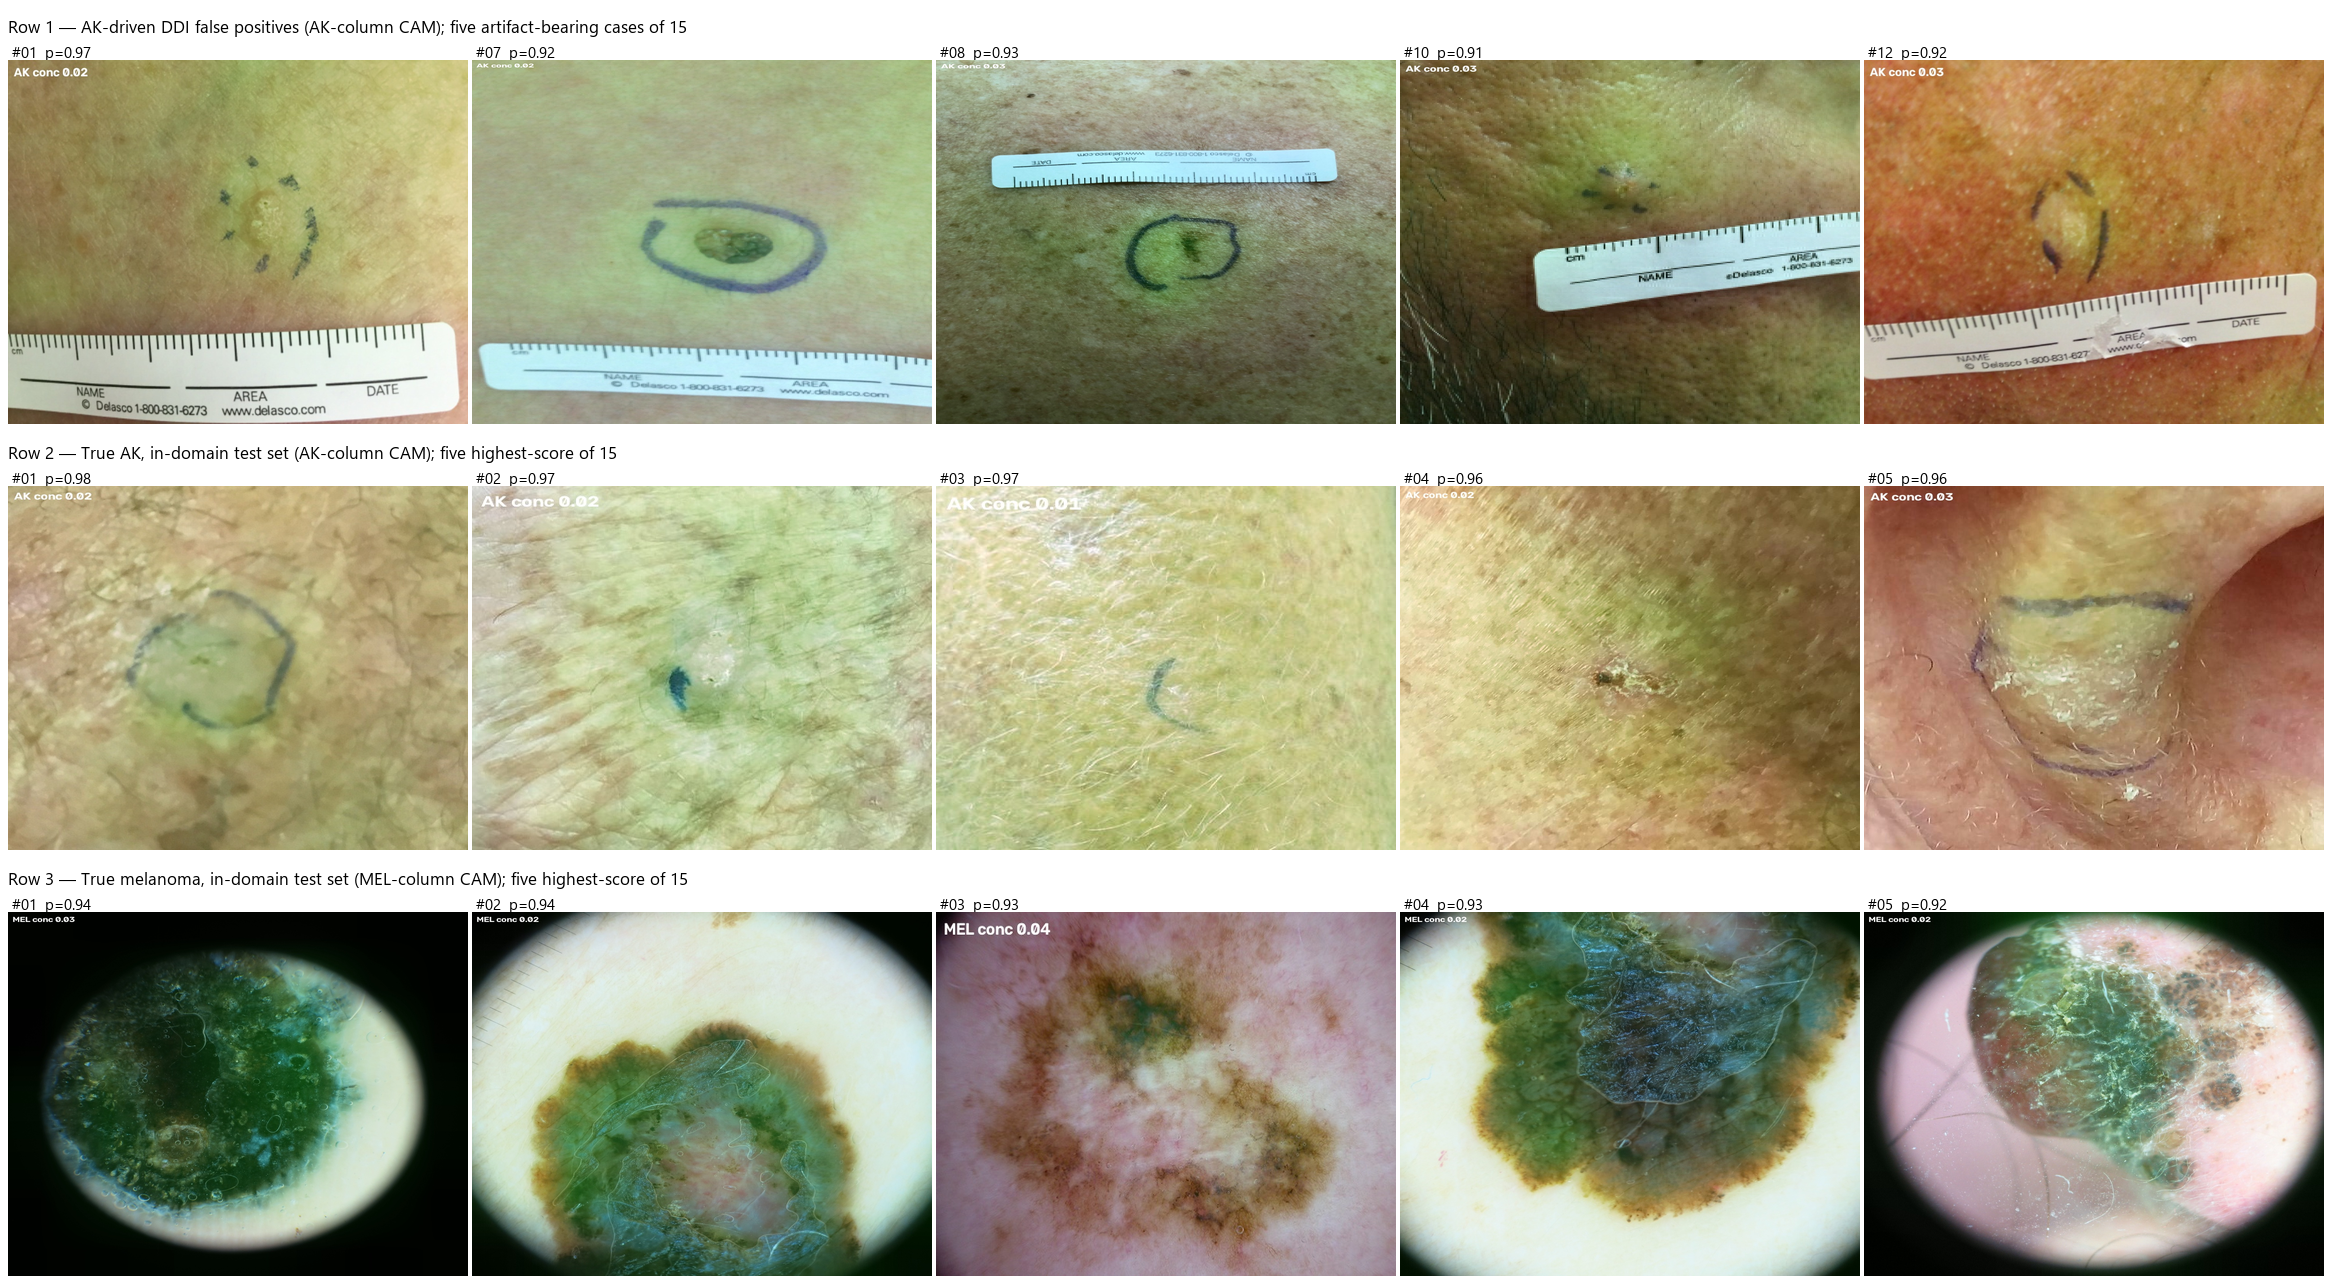
\includegraphics[width=\textwidth]{figs/fig_cam_grid.png}
\caption{Grad-CAM overlays for the three cohorts (per-tile labels: rank, malignant probability). Row~1: the five false positives whose capture artifacts (paper rulers, surgical ink) are attested in the authors' artifact key -- five of the fifteen flagged cases, all showing the same field-wide activation. Rows~2--3: the five highest-scoring true-AK and true-melanoma comparators. Both AK cohorts activate field-wide; the melanoma comparators are dermoscopic acquisitions whose lesion-localized appearance partly reflects capture modality (modality-controlled analysis in the text).}
\label{fig:camgrid}
\end{figure*}

\subsection{Domain Shift, Not Skin Tone, Drives the Artifact}
Within DDI, benign-image AK probability is nearly flat across tone groups and
\emph{highest} for the lightest-tone group (FST~I--II 0.440, FST~V--VI 0.371,
FST~III--IV 0.318) -- the opposite of a monotone tone gradient. At identical
self-reported tone (FST~I--II), DDI benigns show AK mean 0.440 vs test-panel
0.043 (KS $=0.78$). We therefore frame the DDI disparity as a
\emph{domain-generalization failure that disproportionately lands on the
group with the weakest underlying ranking signal}: the capture artifact and
the tone-related performance gap compound rather than share a single cause.

\subsection{A Post-Hoc Correction Cannot Repair the Score}
A post-hoc down-weighting $p' = p_{\mathrm{mal}} - \lambda
P_{\mathrm{AK}}$, with $\lambda$ and the decision threshold fitted on one
stratified half of DDI and evaluated once on the held-out half, yields at most
marginal gains: tune-half AUC peaks at $\lambda^*=0.25$ (0.609 vs 0.596
baseline) and degrades monotonically beyond. At $\lambda^*$ the eval-half
specificity is statistically unchanged (0.025 $\to$ 0.025 overall) and the
EO sensitivity gap moves from 0.125 [0.000, 0.250] to 0.083 [0.000,
0.208]. Aggressive deflation ($\lambda=0.8$) destroys in-domain AK detection
(AK-class recall at $\approx$80\% specificity: 0.955 $\to$ 0.444) while
still not fixing DDI specificity. The failure is structural: on eval-half
benign images, deflating AK merely migrates the dominant malignant contributor
to other columns (argmax share AK 62.3\% $\to$ 28.3\%, BCC 15.6\%
$\to$ 29.9\%, MEL 16.4\% $\to$ 23.0\% at $\lambda=0.8$) --
single-column recalibration is whack-a-mole when the shared representation maps
the capture domain itself onto malignancy. The deficit is therefore
representational: closing it requires in-domain training signal (fine-tuning
with DDI-style images, including hard negatives, and tone/capture
augmentation), not score- or threshold-level correction.
%% === END STEP3-SECTION ===

\section{Discussion}
\subsection{Why Fairness Failures Were Silent}
None of the three defects produced an exception during training or degraded top-line test accuracy (73.7\% balanced accuracy was unaffected by any of them). Each was detectable only by (a) tracing a derived quantity back to its taxonomy source of truth, (b) inspecting the empirical distribution of an auxiliary label rather than trusting its presence, and (c) inspecting per-tensor quantization statistics rather than only end-to-end accuracy. We argue this generalizes: fairness and calibration code paths are exercised far less often than the primary training loop and are correspondingly more likely to harbor silent, high-impact bugs.

\subsection{Retraining Alone Does Not Fix a Fairness Gap Rooted in Label Corruption}
A na\"ive response to a 25\% cross-tone fairness gap is to train longer. We show this would have been ineffective: the gap originated in corrupted \emph{supervision}, not insufficient optimization -- the label-choice bias mechanism documented by Obermeyer et al.~\cite{obermeyer2019}, and a dataset-shift hazard of the kind catalogued by Finlayson et al.~\cite{finlayson2021}. Correcting the label source is a prerequisite for any fairness-training intervention to have a measurable effect, and should precede, not follow, additional compute expenditure.

\subsection{Domain Shift and the Limits of Post-Hoc Fairness Repair}
The DDI analysis (Section~\ref{sec:step3}) adds a fourth lesson: post-hoc repairs (per-group thresholds, single-column recalibration) cannot fix a representational domain gap, and attention-map morphology alone cannot diagnose one -- matched-comparator Grad-CAM analysis showed the diffuse activation previously read as an artifact signature is in fact the head's normal behavior. Given this representational deficit, we deliberately did not attempt in-domain fine-tuning in this work: Sections \ref{sec:threshold} and \ref{sec:step3} establish that every score- and threshold-level correction fails, so we identify targeted data acquisition (DDI-style capture-domain images, including benign hard negatives) and score-level fine-tuning under the corrected tone supervision as the appropriate future work, to be judged against the per-group ROC ceilings reported here.

\subsection{Quantization Choice Is Architecture-Dependent}
GeM pooling's learned exponent is a known source of quantization sensitivity; our finding that it produces an activation scale roughly $10^{3}$-$10^{4}\times$ larger than typical convolutional layers offers a concrete diagnostic (per-tensor scale inspection) for detecting this class of failure before it reaches deployment, and dynamic-range quantization as a practical mitigation when full INT8 is required elsewhere in a pipeline.

\subsection{Limitations}
The post-correction tone distribution remains heavily skewed toward Types II--III (98.8\% of training data), reflecting the true composition of HAM10000/ISIC~2019 rather than a residual bug. We expect the equalized-odds gap to narrow with genuine supervision but not to close without additional dark-skin-tone training data; closing it fully is a data-acquisition problem, not a modeling one. Best validation balanced accuracy (67.8--73.7\% across evaluation protocols) had not converged at the time of writing; retraining to convergence under corrected tone supervision, and re-measuring the DDI fairness gap, is ongoing work. Three caveats attach to the Step~\ref{sec:step3} analysis. First, capture modality is confounded with class in the available data (99\% of test melanomas are dermoscopic acquisitions vs 62\% of AKs), so attention morphology cannot be compared across classes without a modality-matched design; the modality-controlled replication indicates the concentration statistic tracks capture modality, and no class-level morphological claim is made. Second, the AK head's preference for darker-than-scene pixels is left as an open question: the same lean appears in the MEL column on clinical-photo melanomas (median CAM--luminance correlation -0.60, though those cases are low-confidence), which argues against an actinic-damage-specific explanation, but disentangling illumination response from lesion-border shadowing requires pixel-level attribution beyond the scope of this audit. Third, the visual overlay review was performed by the authors rather than an independent dermatologist, so the ruler and artifact counts are manual tallies pending expert confirmation.

\section{Conclusion}
We identified and corrected three independent, silently-compounding defects in a fairness-aware skin lesion classifier: a stale binary-label mapping, fabricated skin-tone training supervision from a swallowed exception, and a catastrophic INT8 quantization failure caused by a learned GeM pooling exponent. Each defect was invisible to standard top-line accuracy monitoring. We provide a corrected, on-device-validated deployment (5.51~MB, clinically calibrated threshold 0.25) and argue that fairness-critical ML pipelines require explicit data-lineage and quantization-scale auditing, not just held-out accuracy, before deployment claims can be trusted.

\begin{thebibliography}{9}
\bibitem{selvaraju2017} R. R. Selvaraju et al., ``Grad-CAM: Visual Explanations from Deep Networks via Gradient-Based Localization,'' \emph{ICCV}, 2017.
\bibitem{hardt2016} M. Hardt, E. Price, N. Srebro, ``Equality of Opportunity in Supervised Learning,'' \emph{NeurIPS}, 2016.
\bibitem{obermeyer2019} Z. Obermeyer, B. Powers, C. Vogeli, S. Mullainathan, ``Dissecting racial bias in an algorithm used to manage the health of populations,'' \emph{Science}, 2019.
\bibitem{finlayson2021} S. G. Finlayson et al., ``The Clinician and Dataset Shift in Artificial Intelligence,'' \emph{N. Engl. J. Med.}, 2021.
\bibitem{ham10000} P. Tschandl, C. Rosendahl, H. Kittler, ``The HAM10000 dataset,'' \emph{Sci. Data}, 2018.
\bibitem{isic2019} ISIC 2019 Challenge Dataset, International Skin Imaging Collaboration.
\bibitem{padufes} A. G. C. Pacheco et al., ``PAD-UFES-20: A skin lesion dataset,'' \emph{Data in Brief}, 2020.
\bibitem{ddi} R. Daneshjou et al., ``Disparities in dermatology AI performance on a diverse, curated clinical image set,'' \emph{Sci. Adv.}, 2022.
\bibitem{gem} F. Radenovi\'c, G. Tolias, O. Chum, ``Fine-tuning CNN Image Retrieval with No Human Annotation,'' \emph{IEEE TPAMI}, 2018.
\end{thebibliography}

\end{document}
